\documentclass[aspectratio=169]{beamer}

\usepackage[utf8]{inputenc}
\usepackage{graphicx}
\usepackage{tikz}
\usetikzlibrary{positioning, arrows.meta, shapes.symbols, decorations.pathreplacing}
\usepackage{pifont}

\usefonttheme{professionalfonts}

% Theme
\usetheme{Madrid}
\definecolor{ucdgreen}{RGB}{0, 102, 51}
\definecolor{gapred}{RGB}{180, 50, 50}
\definecolor{stepfill}{RGB}{230, 243, 235}
\definecolor{donefill}{RGB}{200, 230, 210}
\definecolor{nextfill}{RGB}{255, 240, 200}
\definecolor{vennblue}{RGB}{70, 130, 180}
\definecolor{vennorange}{RGB}{210, 140, 50}
\usecolortheme[named=ucdgreen]{structure}
\setbeamertemplate{navigation symbols}{}
\setbeamersize{text margin left=7mm, text margin right=7mm}

\title[UCD Mathematics PhD Seminar]{}
\author[Lainey Ward]{}
\institute[]{}
\date{}

\begin{document}

% --------------------------------------------------
% SLIDE 1: Hook — Oasis in the Predictability Desert?
% --------------------------------------------------
% PURPOSE: Farmer story, drought-to-flood visual.
%          Script carries the hook, show of hands,
%          and introduces the predictability desert.
% --------------------------------------------------
\begin{frame}{Oasis in the Predictability Desert?}

    \begin{columns}[T, totalwidth=\textwidth]

        % ── Left: Farmer ──────────────────────────────────
        \begin{column}{0.15\textwidth}
            \raggedright
            
\includegraphics[height=4.0cm]{farmer_cropped.png}
        \end{column}

        % ── Centre: Drought → Flood ───────────────────────
        \begin{column}{0.55\textwidth}
            \hspace*{-5mm}%
            \begin{tikzpicture}

                % Drought
                \node[anchor=south] (drought) at (-0.7, 0)
                    {
\includegraphics[height=3.4cm]{drought_cropped.png}};

                % Arrow
                \node[anchor=center] (arrow) at (1.38, 1.5)
                    {
\includegraphics[height=0.7cm]{arrow_cropped.png}};

                % Flood
                \node[anchor=south] (flood) at (3.7, -0.15)
                    {
\includegraphics[height=3.4cm]{flood.png}};

            \end{tikzpicture}
        \end{column}

        % ── Right: S2S timescale label ────────────────────
        \begin{column}{0.28\textwidth}
            \centering\par\vspace{14mm}%
            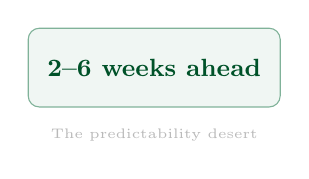
\begin{tikzpicture}[
                tbox/.style={draw=ucdgreen!50, fill=ucdgreen!6,
                    rounded corners=4pt, minimum width=3.2cm,
                    minimum height=1.0cm, align=center,
                    font=\small\bfseries, text=ucdgreen!80!black}
            ]
                \node[tbox] (s2s) at (0, 0)
                    {2--6 weeks ahead};
                \node[font=\tiny, text=gray!55, below=0.15cm of s2s,
                      align=center]
                    {The predictability desert};

            \end{tikzpicture}
        \end{column}

    \end{columns}

\end{frame}

% --------------------------------------------------
% SLIDE 2: The prediction gap
% --------------------------------------------------
% PURPOSE: Mariotti figure shows where S2S sits.
%          Right side explains WHY skill is low here
%          (initial conditions fading, boundary forcings
%          not yet dominant) and the 24% stat.
% --------------------------------------------------
\begin{frame}{Why Is This So Hard to Predict?}

    \begin{columns}[c, totalwidth=\textwidth]

        % ── Left: Mariotti figure ─────────────────────────
        \begin{column}{0.72\textwidth}
            \centering
            
\includegraphics[width=\textwidth, keepaspectratio,
                trim=0 30 0 0, clip]
                {s2s_prediction_gap_mariotti2018.jpg}\\[-0.2em]
            {\tiny\color{gray!50} Source: Mariotti et al.\ (2018)}
        \end{column}

        % ── Right: 24% stat ──────────────────────────────
        \begin{column}{0.26\textwidth}
            \centering
            \vspace{1cm}
            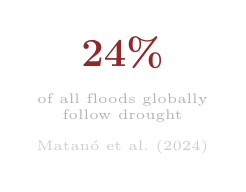
\begin{tikzpicture}
                \node[font=\Large\bfseries, text=gapred!80!black]
                    at (0, 0) {24\%};
                \node[font=\tiny, text=gray!60, align=center]
                    at (0, -0.7) {of all floods globally\\follow drought};
                \node[font=\tiny, text=gray!40]
                    at (0, -1.2) {Matan\'o et al.\ (2024)};
            \end{tikzpicture}
        \end{column}

    \end{columns}

\end{frame}

% --------------------------------------------------
% SLIDE 3: Three literatures, one gap (Venn)
% --------------------------------------------------
% PURPOSE: Show the three research communities and
%          that the centre (the thesis question) is
%          unexplored. Script names the three fields
%          and the pairwise overlaps verbally.
% --------------------------------------------------
\begin{frame}{What Does the Literature Say?}

    \centering
    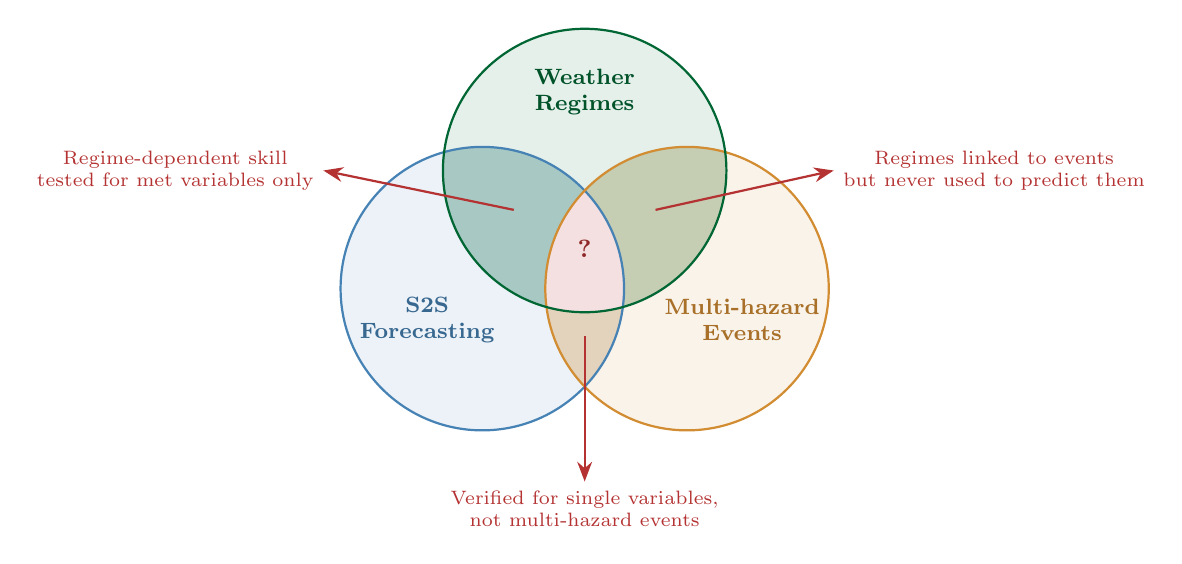
\begin{tikzpicture}
    \def\r{1.8}

    % Base circle fills
    \fill[vennblue!10] (-1.3,0) circle (\r);
    \fill[vennorange!10] ( 1.3,0) circle (\r);
    \fill[ucdgreen!10] (0,1.5) circle (\r);

    % Pairwise overlap fills
    \begin{scope}
      \clip (-1.3,0) circle (\r);
      \clip ( 1.3,0) circle (\r);
      \fill[vennblue!25!vennorange, opacity=0.3] (-3,-3) rectangle (3,3);
    \end{scope}
    \begin{scope}
      \clip (-1.3,0) circle (\r);
      \clip (0,1.5) circle (\r);
      \fill[vennblue!40!ucdgreen, opacity=0.3] (-3,-3) rectangle (3,3);
    \end{scope}
    \begin{scope}
      \clip ( 1.3,0) circle (\r);
      \clip (0,1.5) circle (\r);
      \fill[ucdgreen!40!vennorange, opacity=0.3] (-3,-3) rectangle (3,3);
    \end{scope}

    % Triple intersection fill
    \begin{scope}
      \clip (-1.3,0) circle (\r);
      \clip ( 1.3,0) circle (\r);
      \clip (0,1.5) circle (\r);
      \fill[gapred!15] (-3,-3) rectangle (3,3);
    \end{scope}

    % Circle outlines
    \draw[vennblue, thick] (-1.3,0) circle (\r);
    \draw[vennorange, thick] ( 1.3,0) circle (\r);
    \draw[ucdgreen, thick] (0,1.5) circle (\r);

    % Circle labels
    \node[align=center, text=vennblue!80!black, font=\footnotesize\bfseries]
        at (-2.0,-0.4) {S2S\\Forecasting};
    \node[align=center, text=vennorange!80!black, font=\footnotesize\bfseries]
        at ( 2.0,-0.4) {Multi-hazard\\Events};
    \node[align=center, text=ucdgreen!80!black, font=\footnotesize\bfseries]
        at (0,2.5) {Weather\\Regimes};

    % Centre — the thesis
    \node[align=center, font=\small\bfseries, text=gapred!80!black]
        at (0,0.5) {?};

    % Pairwise gap labels
    % S2S × Multi-hazard (bottom)
    \node[align=center, font=\scriptsize, text=gapred] (g1) at (0,-2.8)
         {Verified for single variables,\\not multi-hazard events};
    \draw[-{Stealth[length=2.5mm]}, thick, gapred] (0,-0.6) -- (g1.north);

    % S2S × Weather Regimes (upper-left)
    \node[align=center, font=\scriptsize, text=gapred] (g2) at (-5.2,1.5)
         {Regime-dependent skill\\tested for met variables only};
    \draw[-{Stealth[length=2.5mm]}, thick, gapred] (-0.9,1.0) -- (g2.east);

    % Weather Regimes × Multi-hazard (upper-right)
    \node[align=center, font=\scriptsize, text=gapred] (g3) at (5.2,1.5)
         {Regimes linked to events\\but never used to predict them};
    \draw[-{Stealth[length=2.5mm]}, thick, gapred] (0.9,1.0) -- (g3.west);

    \end{tikzpicture}

\end{frame}

% --------------------------------------------------
% SLIDE 4: Detection approaches
% --------------------------------------------------
% PURPOSE: Terminology map shows geographic fragmentation
%          of the field. Script explains the two schools
%          (joint indices vs episode-linking) verbally.
% --------------------------------------------------
\begin{frame}{How Do You Detect These Events?}

    \begin{columns}[c, totalwidth=\textwidth]

        \begin{column}{0.75\textwidth}
            
\includegraphics[width=\textwidth]
                {terminology_map.png}
        \end{column}

        \begin{column}{0.23\textwidth}
            \centering
            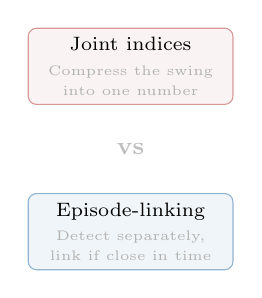
\begin{tikzpicture}[
                vs/.style={font=\small\bfseries, text=gray!50}
            ]

            % Joint indices (red — matches China cluster)
            \node[draw=gapred!50, rounded corners=3pt,
                  minimum width=2.6cm, minimum height=0.9cm,
                  fill=gapred!6, align=center, font=\scriptsize] (ji) at (0, 1.2)
                {Joint indices\\[0.1em]
                 {\tiny\color{gray!60} Compress the swing}\\[-0.1em]
                 {\tiny\color{gray!60} into one number}};

            \node[vs] at (0, 0.15) {vs};

            % Episode-linking (blue — matches US/Europe)
            \node[draw=vennblue!60, rounded corners=3pt,
                  minimum width=2.6cm, minimum height=0.9cm,
                  fill=vennblue!8, align=center, font=\scriptsize] (el) at (0, -0.9)
                {Episode-linking\\[0.1em]
                 {\tiny\color{gray!60} Detect separately,}\\[-0.1em]
                 {\tiny\color{gray!60} link if close in time}};

            \end{tikzpicture}
        \end{column}

    \end{columns}

\end{frame}

% --------------------------------------------------
% SLIDE 5: Pipeline and research questions
% --------------------------------------------------
% PURPOSE: State the two RQs and show the Paper 1
%          pipeline as a chevron chain. Mention Papers
%          2 and 3 briefly. Script carries the detail.
% --------------------------------------------------
\begin{frame}{What Am I Testing?}

    % --- Two research questions ---
    \vspace{-0.3em}
    \begin{enumerate}
        \item[\textcolor{ucdgreen}{\textbf{1.}}] {\itshape How does prediction skill at S2S lead times compare across forecast variables, impact variables, and multi-hazard events?}
        \item[\textcolor{ucdgreen}{\textbf{2.}}] {\itshape Under what atmospheric conditions does this skill emerge?}
    \end{enumerate}

    \vspace{2.0em}

    % --- Pipeline chevron chain ---
    \centering
    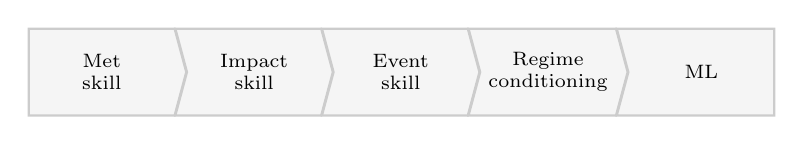
\begin{tikzpicture}[
        xscale=1.0,
        chev/.style={
            minimum width=2.0cm, minimum height=1.1cm,
            align=center, font=\scriptsize, inner sep=3pt,
            signal, signal to=east, signal from=west,
            signal pointer angle=150,
            thick
        },
        plbl/.style={font=\tiny, below=0.15cm}
    ]

    % Met skill
    \node[chev, fill=gray!8, draw=gray!40, text=black,
          signal from=none] (p1) at (0, 0)
        {Met\\skill};

    % Impact skill
    \node[chev, fill=gray!8, draw=gray!40, text=black,
          right=-0.02cm of p1] (p2)
        {Impact\\skill};

    % Event skill
    \node[chev, fill=gray!8, draw=gray!40, text=black,
          right=-0.02cm of p2] (p3)
        {Event\\skill};

    % Regime conditioning
    \node[chev, fill=gray!8, draw=gray!40, text=black,
          right=-0.02cm of p3] (p4)
        {Regime\\conditioning};

    % ML
    \node[chev, fill=gray!8, draw=gray!40, text=black,
          signal to=none, right=-0.02cm of p4] (p5)
        {ML};

    \end{tikzpicture}

    \vspace{3.0em}

    % --- Three papers ---
    \centering
    
\begin{tikzpicture}[
        pbox/.style={draw=ucdgreen!40, thick, rounded corners=4pt,
            minimum width=3.6cm, minimum height=0.9cm,
            fill=ucdgreen!5, align=center, font=\footnotesize}
    ]
    \node[pbox, fill=ucdgreen!6, draw=ucdgreen!60] (pa) at (0, 0)
        {\textbf{Paper 1}\\[-0.1em]
         {\scriptsize Drought-to-flood}};
    \node[pbox, fill=vennorange!8, draw=vennorange!60] (pb) at (4.4, 0)
        {\textbf{Paper 2}\\[-0.1em]
         {\scriptsize Energy source droughts}};
    \node[pbox, fill=vennblue!6, draw=vennblue!60] (pc) at (8.8, 0)
        {\textbf{Paper 3}\\[-0.1em]
         {\scriptsize ANTICIPATE}};
    \end{tikzpicture}

\end{frame}

% --------------------------------------------------
% SLIDE 6: Where ML enters
% --------------------------------------------------
% PURPOSE: Full pipeline from forecast to transition,
%          with ML entry points hanging off the right
%          stages. Script carries the detail.
% --------------------------------------------------
\begin{frame}{Where Does ML Fit?}

    \centering
    \vspace{0.5em}
    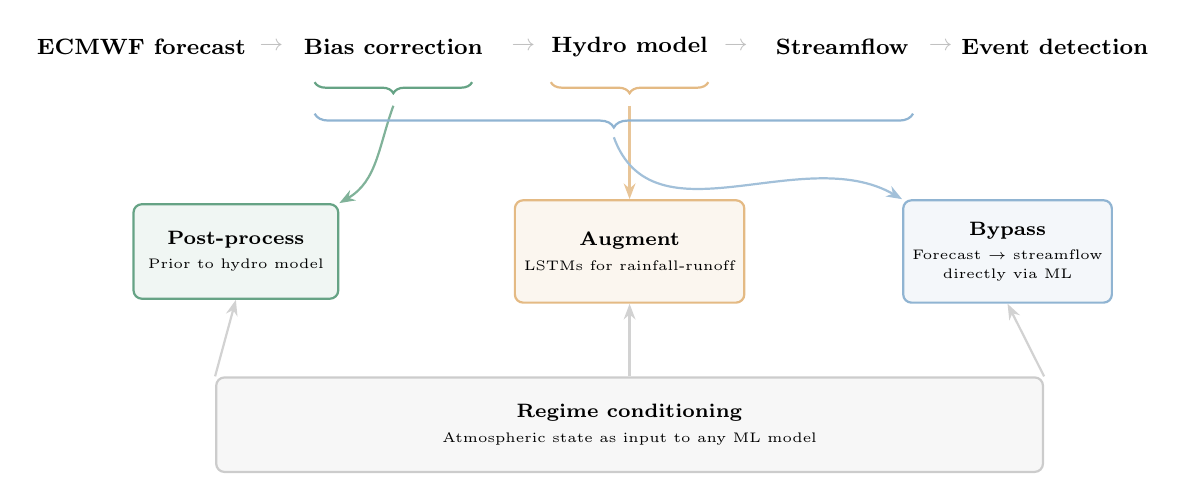
\begin{tikzpicture}[
        plbl/.style={font=\footnotesize\bfseries, text=ucdgreen!80!black},
        parr/.style={font=\footnotesize, text=gray!50},
        mlbox/.style={draw=vennorange!60, thick, rounded corners=3pt,
            minimum width=3.0cm, minimum height=1.3cm,
            fill=vennorange!8, align=center, font=\scriptsize},
        mlarr/.style={-{Stealth[length=2mm]}, thick, vennorange!50}
    ]

    % === Pipeline as text chain (black) ===
    \node[font=\footnotesize\bfseries] (s1) at (0, 3.0) {ECMWF forecast};
    \node[font=\footnotesize, text=gray!50] at (1.65, 3.0) {$\rightarrow$};
    \node[font=\footnotesize\bfseries] (s2) at (3.2, 3.0) {Bias correction};
    \node[font=\footnotesize, text=gray!50] at (4.85, 3.0) {$\rightarrow$};
    \node[font=\footnotesize\bfseries] (s3) at (6.2, 3.0) {Hydro model};
    \node[font=\footnotesize, text=gray!50] at (7.55, 3.0) {$\rightarrow$};
    \node[font=\footnotesize\bfseries] (s4) at (8.9, 3.0) {Streamflow};
    \node[font=\footnotesize, text=gray!50] at (10.15, 3.0) {$\rightarrow$};
    \node[font=\footnotesize\bfseries] (s5) at (11.6, 3.0) {Event detection};

    % === Brace 1: Post-process (green, under Bias correction) ===
    \draw[decorate, decoration={brace, amplitude=4pt, mirror},
          thick, ucdgreen!60]
        (2.2, 2.55) -- (4.2, 2.55);
    \node[draw=ucdgreen!60, thick, rounded corners=3pt,
          minimum width=2.6cm, minimum height=1.2cm,
          fill=ucdgreen!6, align=center, font=\scriptsize] (ml1) at (1.2, 0.4)
        {\textbf{Post-process}\\[0.1em]
         {\tiny Prior to hydro model}};
    \draw[-{Stealth[length=2mm]}, thick, ucdgreen!50]
        (3.2, 2.25) to[out=-110, in=30] (ml1.north east);

    % === Brace 2: Augment (orange, under Hydro model) ===
    \draw[decorate, decoration={brace, amplitude=4pt, mirror},
          thick, vennorange!60]
        (5.2, 2.55) -- (7.2, 2.55);
    \node[mlbox, minimum width=2.6cm] (ml2) at (6.2, 0.4)
        {\textbf{Augment}\\[0.1em]
         {\tiny LSTMs for rainfall-runoff}};
    \draw[mlarr] (6.2, 2.25) to[out=-90, in=90] (ml2.north);

    % === Brace 3: Bypass (blue, from Bias correction through Streamflow) ===
    \draw[decorate, decoration={brace, amplitude=5pt, mirror},
          thick, vennblue!60]
        (2.2, 2.15) -- (9.8, 2.15);
    \node[draw=vennblue!60, thick, rounded corners=3pt,
          minimum width=2.6cm, minimum height=1.3cm,
          fill=vennblue!6, align=center, font=\scriptsize] (ml3) at (11.0, 0.4)
        {\textbf{Bypass}\\[0.1em]
         {\tiny Forecast $\rightarrow$ streamflow}\\[-0.15em]
         {\tiny directly via ML}};
    \draw[-{Stealth[length=2mm]}, thick, vennblue!50]
        (6.0, 1.85) to[out=-70, in=150] (ml3.north west);

    % === Regime conditioning (bottom bar) ===
    \node[draw=gray!40, thick, rounded corners=3pt,
          minimum width=10.5cm, minimum height=1.2cm,
          fill=gray!6, align=center, font=\scriptsize]
        (reg) at (6.2, -1.8)
        {\textbf{Regime conditioning}\\[0.1em]
         {\tiny Atmospheric state as input to any ML model}};

    \draw[-{Stealth[length=2mm]}, thick, gray!35] (reg.north west) -- (ml1.south);
    \draw[-{Stealth[length=2mm]}, thick, gray!35] (reg.north) -- (ml2.south);
    \draw[-{Stealth[length=2mm]}, thick, gray!35] (reg.north east) -- (ml3.south);

    \end{tikzpicture}

\end{frame}

% --------------------------------------------------
% SLIDE 7: Current progress
% --------------------------------------------------
% PURPOSE: EEFH vs SEAS5 comparison. Script explains
%          the two systems and what has been verified.
% --------------------------------------------------
\begin{frame}{Where Am I On This?}

    \begin{columns}[c, totalwidth=\textwidth]

        \begin{column}{0.42\textwidth}

            \centering
            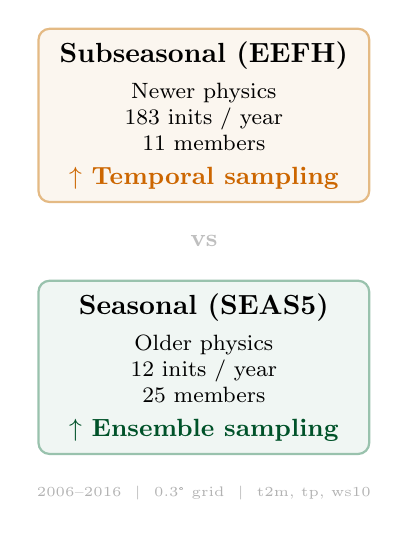
\begin{tikzpicture}[
                sysbox/.style={draw=ucdgreen!40, thick, rounded corners=4pt,
                    minimum width=4.2cm, minimum height=2.2cm,
                    fill=ucdgreen!4, align=center, font=\footnotesize}
            ]
            % EEFH
            \node[sysbox, fill=vennorange!8, draw=vennorange!60] (eefh) at (0, 1.6)
                {\textbf{\normalsize Subseasonal (EEFH)}\\[0.4em]
                 Newer physics\\
                 183 inits / year\\
                 11 members\\[0.3em]
                 {\small\bfseries\color{orange!80!black} $\uparrow$ Temporal sampling}};

            % SEAS5
            \node[sysbox, fill=ucdgreen!6, draw=ucdgreen!40] (seas) at (0, -1.6)
                {\textbf{\normalsize Seasonal (SEAS5)}\\[0.4em]
                 Older physics\\
                 12 inits / year\\
                 25 members\\[0.3em]
                 {\small\bfseries\color{ucdgreen!80!black} $\uparrow$ Ensemble sampling}};

            % vs
            \node[font=\small\bfseries, text=gray!50] at (0, 0) {vs};

            % Setup summary
            \node[font=\tiny, text=gray!60, align=center] at (0, -3.2)
                {2006--2016 ~\textbar~ 0.3\textdegree{} grid ~\textbar~ t2m, tp, ws10};

            \end{tikzpicture}

        \end{column}

        \begin{column}{0.56\textwidth}
            \centering
            % === PLOT PLACEHOLDER ===
            % Replace with \includegraphics when verification
            % figures are ready.
            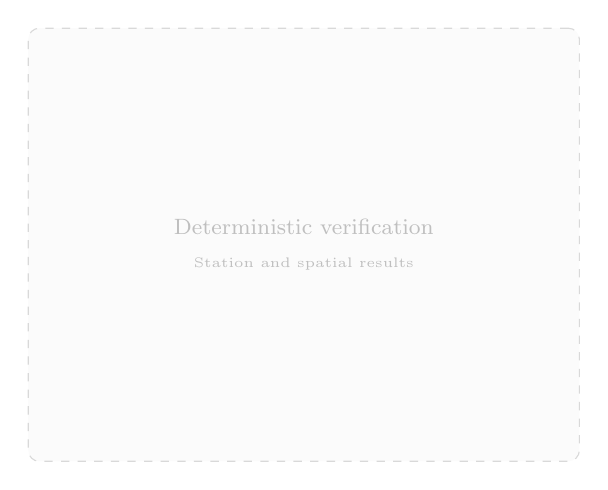
\begin{tikzpicture}
                \node[draw=gray!30, dashed, rounded corners,
                      minimum width=7.0cm, minimum height=5.5cm,
                      fill=gray!3, font=\footnotesize\color{gray!50}, align=center]
                    {Deterministic verification\\[0.3em]
                     {\tiny Station and spatial results}};
            \end{tikzpicture}
        \end{column}

    \end{columns}

\end{frame}

% --------------------------------------------------
% SLIDE 8: Conclusions
% --------------------------------------------------
% PURPOSE: Shown after "Before I conclude, does anyone
%          have any questions?" and the Q&A. Concise
%          bullet-point wrap-up.
% --------------------------------------------------
\begin{frame}{Conclusions}

    \vspace{1.5em}
    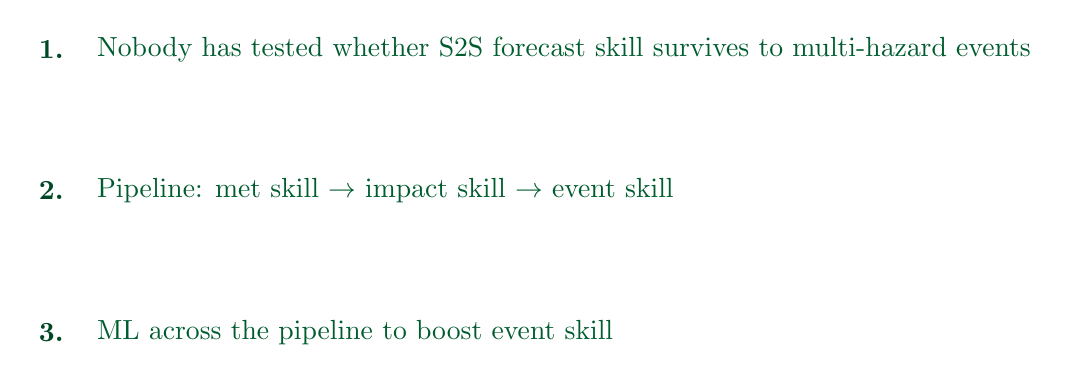
\begin{tikzpicture}[
        bul/.style={font=\normalsize, text=ucdgreen!90!black,
                    anchor=west},
        num/.style={font=\normalsize\bfseries, text=ucdgreen!70!black,
                    anchor=east, minimum width=0.6cm}
    ]

    \node[num] at (0, 0) {1.};
    \node[bul] at (0.15, 0)
        {Nobody has tested whether S2S forecast skill survives to multi-hazard events};

    \node[num] at (0, -1.8) {2.};
    \node[bul] at (0.15, -1.8)
        {Pipeline: met skill $\rightarrow$ impact skill $\rightarrow$ event skill};

    \node[num] at (0, -3.6) {3.};
    \node[bul] at (0.15, -3.6)
        {ML across the pipeline to boost event skill};

    \end{tikzpicture}

\end{frame}

\end{document}
